\documentclass[11pt]{article}

\usepackage{amsmath,amssymb,amsthm}
\usepackage[margin=1.1in]{geometry}
\usepackage{booktabs}
\usepackage{graphicx}
\usepackage{algorithm}
\usepackage{algpseudocode}
\usepackage[colorlinks=true,linkcolor=blue,citecolor=blue,urlcolor=blue]{hyperref}

\graphicspath{{../experiments/out/}}

\newtheorem{theorem}{Theorem}[section]
\newtheorem{proposition}[theorem]{Proposition}
\newtheorem{lemma}[theorem]{Lemma}
\newtheorem{corollary}[theorem]{Corollary}
\theoremstyle{definition}
\newtheorem{definition}[theorem]{Definition}
\newtheorem{remark}[theorem]{Remark}
\newtheorem{measured}[theorem]{Measured Result}

\newcommand{\R}{\mathbb{R}}
\newcommand{\norm}[1]{\left\lVert #1 \right\rVert}
\newcommand{\ROF}{\mathrm{ROF}}
\newcommand{\PG}{P_{G_\mu}}
\newcommand{\dv}{\operatorname{div}}

\title{Transport Geometry Fusion Descent:\\
a sub-second implementation of Meyer's $G$-norm\\
cartoon + texture decomposition}
\author{Joshuah Rainstar\\
\texttt{joshuah.rainstar@gmail.com}}
\date{July 21, 2026}

\begin{document}
\maketitle

\begin{abstract}
Gilles and Osher solve Meyer's cartoon + texture decomposition by an outer
alternation whose inner problems are Rudin--Osher--Fatemi (ROF) solves,
implemented with Split Bregman iterations. We show that their Algorithm~3 is
exactly a two-projector alternation between a total-variation smoothing and
the projection onto Meyer's $G$-ball. We then present transport geometry
fusion descent (TGFD), which replaces the nested outer loop with interleaved
single Bregman sweeps against persistent auxiliary states. On the $512^2$
Barbara image used by Gilles and Osher, TGFD reproduces the decomposition
reached by the nested algorithm in 361 seconds to a relative distance of
$10^{-2}$, without visible difference, in 0.9 seconds. We establish three
quantitative laws governing acceleration in this problem. First, a momentum
polarity: heavy-ball extrapolation of the primal iterates diverges for
$\beta\ge0.8$, whereas the same impulse applied to the dual flux --- the
field $p$ in Meyer's definition $v=\dv p$ --- accelerates Chambolle's
projector by a factor of 40 at equal iteration count. Second, a scope law
for warm starts: Bregman auxiliary fields transfer across outer passes of
one subproblem but not across fidelity constants. Third, a soft-rung law
for scale decompositions on the $G$-axis: the capture fraction of an
oscillation under the $G$-ball projection is a linear ramp of 10--90\%
width $9$--$14\times$ in $\mu$, so that ROF scale ladders are graded rather
than cellular, admit no critical rung ratio, and support approximately two
separable texture bands per image. A three-rung ladder nevertheless
isolates the contour-leakage artifact of the single-$\mu$ decomposition
into its coarsest band, yielding a textile band that no single-$\mu$
decomposition produces. We conclude with an account of the measured
principles, obtained in a precursor program on time-frequency
super-resolution, from which the method derives.
\end{abstract}

\section{Introduction}

The cartoon + texture model of Meyer \cite{meyer} decomposes an image $f$
into a bounded-variation component $u$ and an oscillatory component $v$
constrained to the ball $G_\mu=\{v:\norm{v}_G\le\mu\}$ of the $G$-norm,
\begin{equation}
\norm{v}_G \;=\; \inf\bigl\{\,\norm{\,|p|\,}_\infty \;:\; v=\dv p \bigr\},
\label{eq:gnorm}
\end{equation}
the infimum taken over vector fields $p$ whose divergence generates $v$.
Aujol, Aubert, Blanc-F\'eraud and Chambolle \cite{aujol} made the model
computable by alternating two subproblems, each solved with Chambolle's
projection algorithm \cite{chambolle}. Gilles and Osher \cite{gilles}
replaced the inner projector with Split Bregman ROF solves \cite{goldstein}
and observed a substantial reduction in inner iterations. The outer loop of
\cite{gilles} --- initialization at $u_0=v_0=0$, inner solves to tolerance,
alternation to convergence --- is inherited unchanged from \cite{aujol}.

We use the model, the inner solver, the test image, and the parameter roles
of \cite{gilles}, and we revise the outer computation. The contributions
are the following.

\begin{enumerate}
\item A reduction (Proposition~\ref{prop:reduction}): Algorithm~3 of
\cite{gilles} is exactly the alternation
$u\leftarrow\ROF(f-v,\lambda)$, $v\leftarrow\PG(f-u)$.
\item A method (Algorithm~\ref{alg:tgfd}): transport geometry fusion
descent, an interleaved single-sweep form of that alternation. On the rig
of Section~\ref{sec:protocol} it reaches a lower fixed-point residual than
the nested algorithm at $26\times$ fewer inner sweeps; on the $512^2$
Barbara image it reproduces the nested decomposition to
$\norm{\Delta u}/\norm{f}=1.0\times10^{-2}$ at a $\sim$400$\times$
reduction in wall time.
\item A momentum polarity law (Section~\ref{sec:polarity}): primal
heavy-ball extrapolation diverges, while FISTA extrapolation of the dual
flux accelerates the texture projection by a factor of 40; momentum carried
across a changing objective is harmful on both sides of the duality gap.
\item A soft-rung law (Section~\ref{sec:softrung}): the $G$-ball capture
curve of an oscillation is a linear ramp, with the consequences that
two-way band routing depends only on the straddling rung, that optimal rung
placement is skewed toward the finer texture, and that the $G$-axis
supports approximately two separable texture bands per image.
\item A band decomposition of the Barbara texture layer
(Section~\ref{sec:quarantine}) in which the contour-leakage artifact of the
single-$\mu$ model concentrates in the coarsest band.
\item An account of the measured principles from which the method derives
(Section~\ref{sec:origins}), stated so that the present paper is
self-contained.
\end{enumerate}

All quantitative claims are measurements obtained under the protocol of
Section~\ref{sec:protocol}; the mathematics required to reproduce them is
contained in Sections~\ref{sec:prelim}--\ref{sec:protocol}.

\section{Preliminaries and discretization}
\label{sec:prelim}

Images are arrays in $[0,255]^{N\times M}$, treated as real-valued with
periodic boundary conditions. The discrete gradient uses forward
differences,
\[
(\nabla u)_{i,j} = \bigl(u_{i,j+1}-u_{i,j},\; u_{i+1,j}-u_{i,j}\bigr),
\]
indices modulo the array dimensions; the divergence is its negative
adjoint,
$(\dv p)_{i,j} = p^x_{i,j}-p^x_{i,j-1} + p^y_{i,j}-p^y_{i-1,j}$.
The total variation is the isotropic sum
$J(u)=\sum_{i,j}\,\bigl|(\nabla u)_{i,j}\bigr|$. The composition
$\Delta=\dv\nabla$ is diagonalized by the discrete Fourier transform with
symbol
\begin{equation}
\hat\Delta(k,l) \;=\; 2\cos(2\pi k/N)-2 \;+\; 2\cos(2\pi l/M)-2 \;\le\; 0.
\label{eq:symbol}
\end{equation}

\paragraph{ROF and the $G$-ball projection.}
For a fidelity coefficient $c>0$ we write
\[
\ROF(g,c) \;=\; \arg\min_w\; J(w)+\tfrac{c}{2}\norm{g-w}_2^2 .
\]
Chambolle's identity \cite{chambolle} states that the ROF residual is the
projection onto the $G$-ball of radius $1/c$:
\begin{equation}
g-\ROF(g,c) \;=\; P_{G_{1/c}}(g).
\label{eq:chambolle}
\end{equation}

\paragraph{The Split Bregman sweep.}
Split Bregman \cite{goldstein} solves $\ROF(g,c)$ by introducing
$d\approx\nabla u$ with penalty $\eta$ and Bregman field $b$. One sweep
against the state $(d,b)$ consists of
\begin{align}
u &\;\leftarrow\; \mathcal{F}^{-1}\!\left[
\frac{c\,\hat g - \eta\,\widehat{\dv(d-b)}}{\,c-\eta\hat\Delta\,}\right],
\label{eq:sbu}\\
t &\;=\;\nabla u + b,\qquad
d \;\leftarrow\; \max\bigl(|t|-\tfrac1\eta,\,0\bigr)\,\frac{t}{|t|},
\label{eq:sbshrink}\\
b &\;\leftarrow\; b+\nabla u-d,
\label{eq:sbb}
\end{align}
where $\mathcal F$ denotes the FFT, the shrinkage \eqref{eq:sbshrink} is
isotropic in the two gradient components, and the linear solve
\eqref{eq:sbu} is exact by \eqref{eq:symbol}. One sweep is the unit of
computational cost throughout this paper.

\paragraph{The dual flux and fast gradient projection.}
The dual of $\ROF(g,c)$ is a constrained least-squares problem in the flux
variable of \eqref{eq:gnorm}:
\begin{equation}
p^\star=\arg\min_{|p|\le1}\;\norm{\,g+\dv p/c\,}_2^2,
\qquad u = g+\dv p^\star/c .
\label{eq:dual}
\end{equation}
Projected gradient descent on \eqref{eq:dual} with step $c/8$ is
Chambolle's algorithm; adding FISTA extrapolation of $p$ yields fast
gradient projection (FGP) \cite{beck}: with $t_0=1$,
\begin{align}
y_k &= p_k + \tfrac{t_{k-1}-1}{t_k}\,(p_k-p_{k-1}),\qquad
u_k = g+\dv y_k/c,\notag\\
p_{k+1} &= \Pi\bigl(y_k+\tfrac{c}{8}\nabla u_k\bigr),\qquad
t_{k+1}=\tfrac{1+\sqrt{1+4t_k^2}}{2},
\label{eq:fgp}
\end{align}
where $\Pi$ is the pointwise projection onto the isotropic unit ball.

\section{Reduction of the Gilles--Osher algorithm}

In \cite{gilles} the operator $\mathrm{P}_{\ROF}(g,c)$ denotes the ROF
solution with fidelity coefficient $c$; this convention is fixed by the
proof of their Proposition~2. Their Algorithm~3 iterates
\[
u_{n+1}=\mathrm{P}_{\ROF}(f-v_n,\lambda),\qquad
v_{n+1}=f-u_{n+1}-\tfrac{1}{\lambda}\,
\mathrm{P}_{\ROF}\!\bigl(\lambda(f-u_{n+1}),\tfrac{1}{\lambda\mu}\bigr).
\]

\begin{proposition}
\label{prop:reduction}
Algorithm 3 of \cite{gilles} is identical to the two-projector alternation
\begin{equation}
u_{n+1}=\ROF(f-v_n,\lambda),\qquad
v_{n+1}=\PG(f-u_{n+1}).
\label{eq:alternation}
\end{equation}
\end{proposition}

\begin{proof}
Substituting $w=\lambda z$ in the objective of the texture step gives
$J(w)+\tfrac{1}{2\lambda\mu}\norm{\lambda g-w}_2^2
=\lambda\bigl[J(z)+\tfrac{1}{2\mu}\norm{g-z}_2^2\bigr]$, whence
$\tfrac{1}{\lambda}\mathrm{P}_{\ROF}(\lambda g,\tfrac{1}{\lambda\mu})
=\ROF(g,\tfrac{1}{\mu})$. The texture update is therefore
$g-\ROF(g,\tfrac1\mu)=\PG(g)$ by \eqref{eq:chambolle}.
\end{proof}

Equation \eqref{eq:alternation} exposes the transfer mechanics of the outer
loop. The cartoon step removes from $u$ a component of $G$-norm at most
$1/\lambda$; the texture step assigns to $v$ whatever portion of $f-u$ lies
within the $\mu$-ball. A clean decomposition requires $1/\lambda$ well
below the $G$-norm of the texture, and under that condition the outer loop
is a geometric transfer of texture mass from $u$ to $v$ at a rate limited
by the sliver size $1/\lambda$. The alternation is therefore an instance of
constraint-family fusion on a single latent image, a structure whose
computational behavior we had previously characterized in the setting
described in Section~\ref{sec:origins}. The principles measured there
transfer to \eqref{eq:alternation}, with polarities that the convexity of
the present problem reverses in specific and instructive ways.

\section{Transport geometry fusion descent}
\label{sec:method}

\begin{algorithm}[t]
\caption{Transport geometry fusion descent (TGFD)}
\label{alg:tgfd}
\begin{algorithmic}[1]
\State $u\gets 0$, $v\gets 0$; Bregman states $(d_u,b_u)\gets0$, $(d_v,b_v)\gets0$
\While{the wall-time budget remains}
  \State apply one sweep \eqref{eq:sbu}--\eqref{eq:sbb} for $\ROF(f-v,\lambda)$, $\eta=2\lambda$, against $(d_u,b_u)$; obtain $u$
  \State apply one sweep \eqref{eq:sbu}--\eqref{eq:sbb} for $\ROF(f-u,1/\mu)$, $\eta=10/\mu$, against $(d_v,b_v)$; obtain $w$
  \State $v \gets (f-u)-w$
\EndWhile
\end{algorithmic}
\end{algorithm}

The method is stated in Algorithm~\ref{alg:tgfd}. Each outer pass performs
one Split Bregman sweep on each subproblem of \eqref{eq:alternation},
against auxiliary fields that persist for the life of the loop. There is no
inner tolerance, no nesting, no momentum, no seed, and no continuation
schedule. The texture-side penalty is $\eta=10/\mu$ rather than the
customary $2c$; at weak fidelity this value is the accuracy-per-sweep
optimum among the settings we tested (Table~\ref{tab:t1}).

Each component absent from Algorithm~\ref{alg:tgfd} was implemented,
measured, and removed on the evidence.

\begin{itemize}
\item \emph{Nesting.} Inner solves to tolerance expend sweeps at outer
states that are still far from the fixed point. Removing the nesting
reduces cost by a factor of approximately 26 at equal or better fixed-point
residual (Table~\ref{tab:iters}).
\item \emph{Primal momentum.} Heavy-ball extrapolation of $(u,v)$ is
neutral for $\beta\le0.6$ and divergent beyond $\beta\approx0.8$
(Section~\ref{sec:polarity}).
\item \emph{Seeding.} A separate initialization pass is redundant: under
single-sweep interleaving from zero, the early passes execute against a
coarse auxiliary state and perform the function of a seed. Explicit seeds
of 5 and 40 sweeps produced no measurable improvement.
\item \emph{Over-relaxation, continuation, multiresolution.}
Krasnosel'ski\u{\i}--Mann relaxation with $\omega\in[1.3,1.9]$, geometric
$\lambda$-continuation from $\lambda/4$ through $\lambda/16$, and a
half-resolution initialization were each tested at fixed wall budget; all
lie within measurement noise of Algorithm~\ref{alg:tgfd}
(Section~\ref{sec:results}), and the half-resolution variant is measurably
worse on Barbara, where downsampling destroys texture near the Nyquist
frequency before the full-resolution passes can restore it.
\end{itemize}

\section{Experimental protocol}
\label{sec:protocol}

\paragraph{Synthetic scene.}
The controlled experiments use a $256^2$ scene with known ground truth on
the grid $(x,y)\in\{0,\dots,n-1\}^2$, $n=256$. The cartoon component is the
affine field $90+40x/n+20y/n$, overwritten by a disk of center
$(0.32n,0.34n)$ and radius $0.18n$ carrying the value $170-30y/n$, and by
the rectangle $[0.55n,0.9n]\times[0.55n,0.85n]$ carrying the value 60. Two
texture components are added, each of the form
$a\,m(x,y)\cos\!\bigl(2\pi(x\cos\theta+y\sin\theta)/T\bigr)$ with amplitude
$a=20$ and window $m=\max(0,1-\rho)^{1/2}$, $\rho$ the distance to the
window center in units of $0.3n$: a coarse texture with $T=12$,
$\theta=0.4$, centered at $(0.38,0.62)n$, and a fine texture with $T=3$,
$\theta=1.2$, centered at $(0.62,0.40)n$. The $G$-norms of the textures are
approximately $a T/2\pi = 38.2$ and $9.5$. Unless stated otherwise,
$\lambda=0.05$ and $\mu=60$ on the synthetic scene, and $\lambda=0.05$,
$\mu=40$ on Barbara ($512^2$, 8-bit grayscale, values scaled to $[0,255]$).

\paragraph{Reference fixed point.}
Errors are measured against a reference computed by 120 exact outer
alternations of \eqref{eq:alternation}, each subproblem solved by 2000 FGP
iterations \eqref{eq:fgp}. The residual drift of this reference over its
final 60 alternations is $2.0\times10^{-3}$ relative to $\norm{f}$, which
is therefore the resolution floor of every comparison below.

\paragraph{Metrics.}
The fixed-point residual of a pair $(u,v)$ is
\[
r(u,v)\;=\;\max\bigl(\norm{u-\ROF(f-v,\lambda)}_2,\;
\norm{v-\PG(f-u)}_2\bigr)\big/\norm{f}_2,
\]
with the two operators evaluated by high-accuracy solves. PSNR is computed
with peak 255. Cost is reported in sweeps and in single-core NumPy seconds;
no compiled code and no GPU are used.

\section{Results}
\label{sec:results}

\begin{table}[t]
\centering
\caption{Synthetic scene, $\lambda=0.05$, $\mu=60$.}
\label{tab:iters}
\begin{tabular}{lrrrrr}
\toprule
variant & sweeps & wall & $r(u,v)$ & PSNR $u$ & PSNR $v$\\
\midrule
Algorithm 3 of \cite{gilles}, nested, tol $10^{-4}$ & 21{,}071 & 18.7\,s & $2.4\times10^{-3}$ & 35.01 & 36.21\\
TGFD, 800 passes & 800 & 0.96\,s & $2.0\times10^{-3}$ & 34.55 & 35.66\\
TGFD + primal heavy-ball $\beta=0.88$ & 800 & 0.85\,s & $5.9\times10^{-2}$ & 27.86 & 24.52\\
\bottomrule
\end{tabular}
\end{table}

Table~\ref{tab:iters} contains the central comparison. TGFD reaches a lower
fixed-point residual than the nested algorithm at $26\times$ fewer sweeps,
and converges to the same decomposition: the relative distance
$\norm{u_{\mathrm{TGFD}}-u_{\mathrm{nested}}}/\norm{f}$ is
$9\times10^{-3}$, within a factor of five of the reference drift floor. The third row
demonstrates that the single mechanism added to the alternation --- primal
momentum --- is the mechanism that degrades it.

\begin{measured}[Barbara, $512^2$, $\lambda=0.05$, $\mu=40$]
\label{mr:barbara}
Nested Algorithm 3 at tolerances $10^{-5}$ requires 63{,}633 sweeps and
361\,s. TGFD at a 0.9-second budget completes 60 passes and reaches
$\norm{u-u_{\mathrm{nested}}}/\norm{f}=1.0\times10^{-2}$, a
$\sim$400$\times$ reduction in wall time; a 2.5-second budget reaches
$5.8\times10^{-3}$. The difference of the two cartoons is an edge-adjacent
ripple visible only under $20\times$ amplification
(Figure~\ref{fig:barbara}). For context, a single texture-side projection
computed with Chambolle's algorithm at tolerance $10^{-4}$ requires 4000
iterations of \eqref{eq:dual}; the inner-solver comparison of \cite{gilles}
is thereby reproduced in passing.
\end{measured}

\begin{figure}[t]
\centering
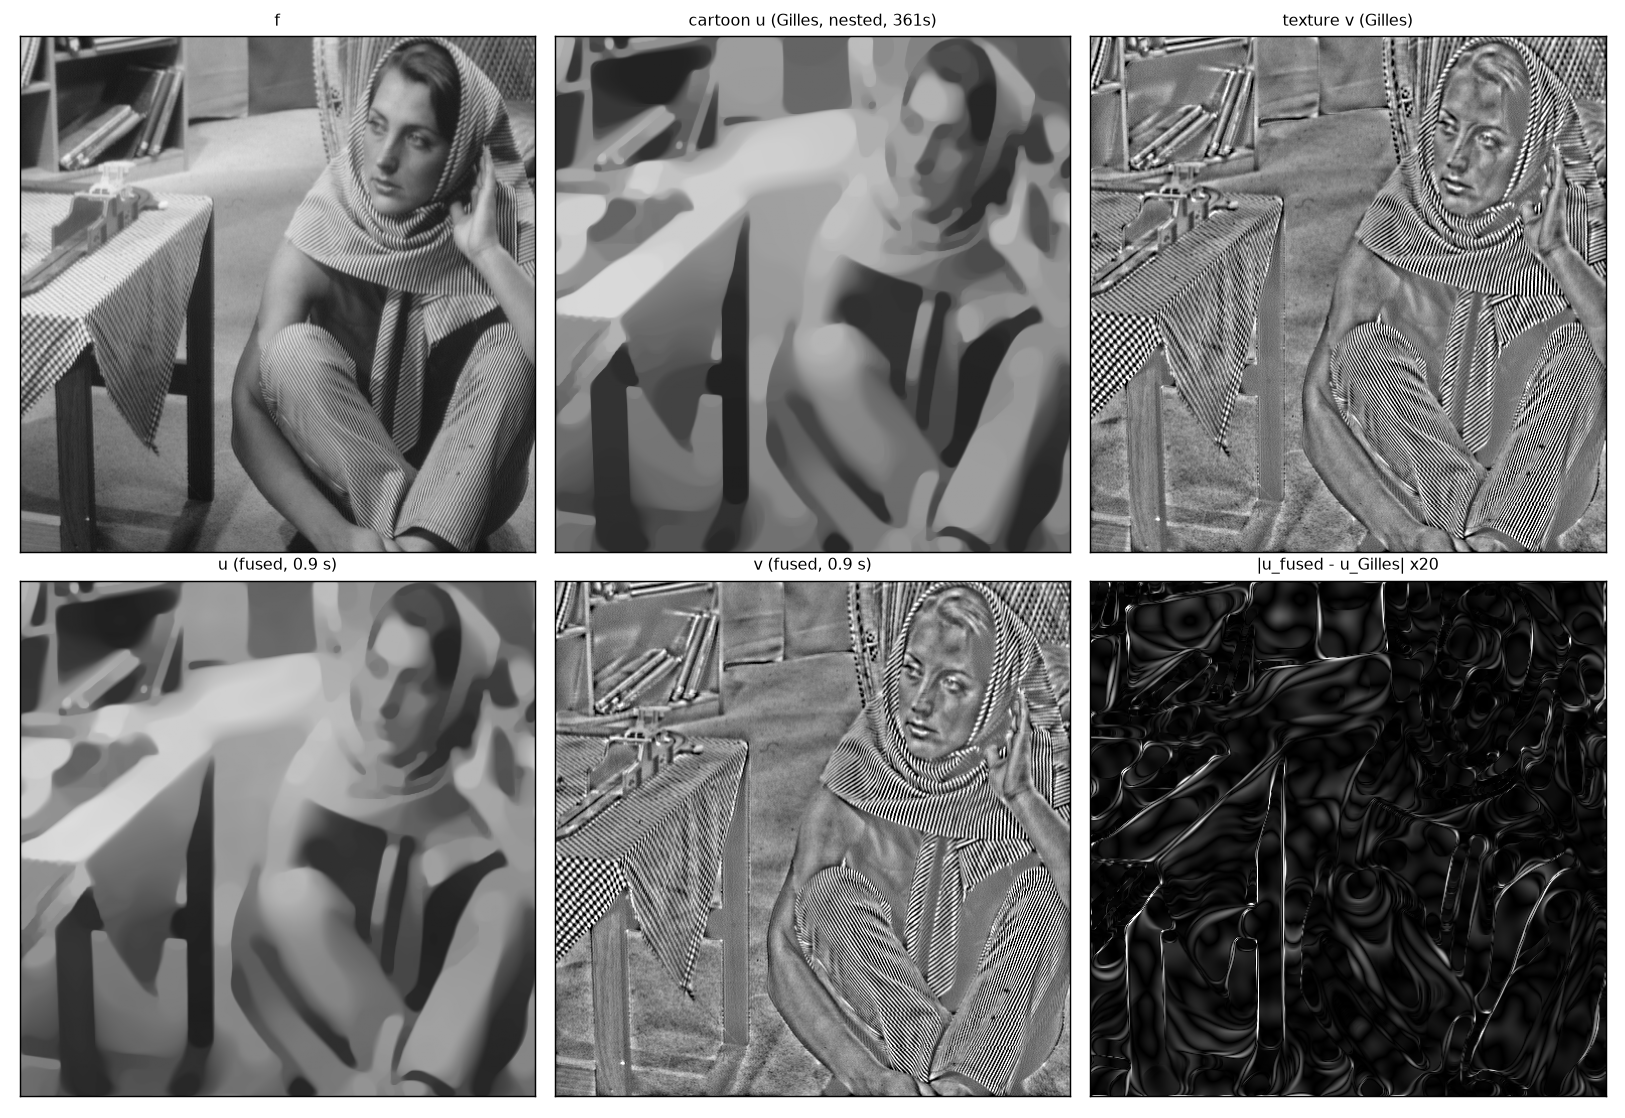
\includegraphics[width=\textwidth]{meyer_barbara.png}
\caption{Barbara. Top row: input; cartoon and texture computed by nested
Algorithm 3 (361\,s). Bottom row: TGFD at a 0.9-second budget; difference
to the nested cartoon, amplified $20\times$.}
\label{fig:barbara}
\end{figure}

A budget study closes the question of further per-pass acceleration at this
scale. With wall time capped at 0.8\,s on the synthetic scene, eleven
variants --- penalty retuning, over-relaxation, continuation, seeding, and
their combinations, as listed in Section~\ref{sec:method} --- produce
errors confined to $[0.9,1.6]\times10^{-2}$ with PSNR $34.1$--$34.5$\,dB.
The decomposition is PSNR-converged by approximately 130 passes; the
residual error beyond that point is outer-transfer distance, and no
per-pass mechanism among those tested removes it. We therefore regard
Algorithm~\ref{alg:tgfd}, without additions, as the operating point of this
problem class at sub-second budgets.

\section{Momentum and the dual flux}
\label{sec:polarity}

Meyer's $G$-norm \eqref{eq:gnorm} is a transport norm: the texture is the
divergence of a flux field, and the norm is the least uniform bound on that
flux. The dual problem \eqref{eq:dual} shows that the ROF subproblems of
\eqref{eq:alternation} are themselves optimizations over the same flux. The
name of the method records this geometry: the quantities that move mass
between the layers of the decomposition, and the quantities that accept
acceleration, are the fluxes rather than the images.

\begin{table}[t]
\centering
\caption{Texture projection at weak fidelity ($c=1/60$): relative error to
the converged projection after 800 inner iterations, and per-iteration
cost.}
\label{tab:t1}
\begin{tabular}{lrr}
\toprule
solver & error @ 800 it & ms/it\\
\midrule
Chambolle iteration on \eqref{eq:dual} & $1.9\times10^{-1}$ & 0.31\\
FGP \eqref{eq:fgp}: the same iteration with flux extrapolation & $5.1\times10^{-3}$ & 0.46\\
Split Bregman, $\eta=2c$ & $3.1\times10^{-2}$ & 0.82\\
Split Bregman, $\eta=10c$ & $4.0\times10^{-3}$ & 0.80\\
\bottomrule
\end{tabular}
\end{table}

\begin{measured}[Momentum polarity]
\label{mr:polarity}
Heavy-ball extrapolation of the primal iterates of \eqref{eq:alternation}
is neutral for $\beta\le0.6$ and divergent for $\beta\ge0.8$: the
fixed-point residual moves from $2.0\times10^{-3}$ at $\beta=0$ to
$2.7\times10^{-2}$ at $\beta=0.8$ and $5.9\times10^{-2}$ at $\beta=0.88$.
The same impulse applied to the dual flux --- FISTA extrapolation of $p$ in
\eqref{eq:fgp} --- reduces the error of the texture projection by a factor
of 40 at equal iteration count relative to the identical iteration without
extrapolation (Table~\ref{tab:t1}).
\end{measured}

\begin{measured}[Stale transport momentum]
\label{mr:stale}
Within the full alternation, where each pass changes the subproblem
objective, carrying the FISTA extrapolation state across passes yields
pipeline error $7.6\times10^{-2}$; carrying the flux while restarting the
extrapolation sequence each pass yields $1.9\times10^{-2}$. Momentum
constructed for one transport flow misdirects the next. Together with
Measured Result~\ref{mr:polarity}, this identifies a single phenomenon
appearing on both sides of the duality gap.
\end{measured}

The same scope law governs the warm state itself. The Bregman fields
$(d,b)$ transfer across outer passes of one subproblem; they do not
transfer across fidelity constants, being $\eta$- and $c$-scaled, and a
state carried to a different constant pins the new solve at the old fixed
point. Within the full pipeline at equal wall time, the Split Bregman
interleave retains the advantage over pure flux iteration
($1.1\times10^{-2}$ against $1.9\times10^{-2}$): the FFT step
\eqref{eq:sbu} solves its linear subproblem exactly once per sweep, and the
$(d,b)$ state carries the edge set of the solution across passes. Flux
acceleration is decisive where a projection must be computed accurately in
isolation --- within Chambolle's projector it should always be used --- while
the pipeline favors the warm interleave.

\begin{figure}[t]
\centering
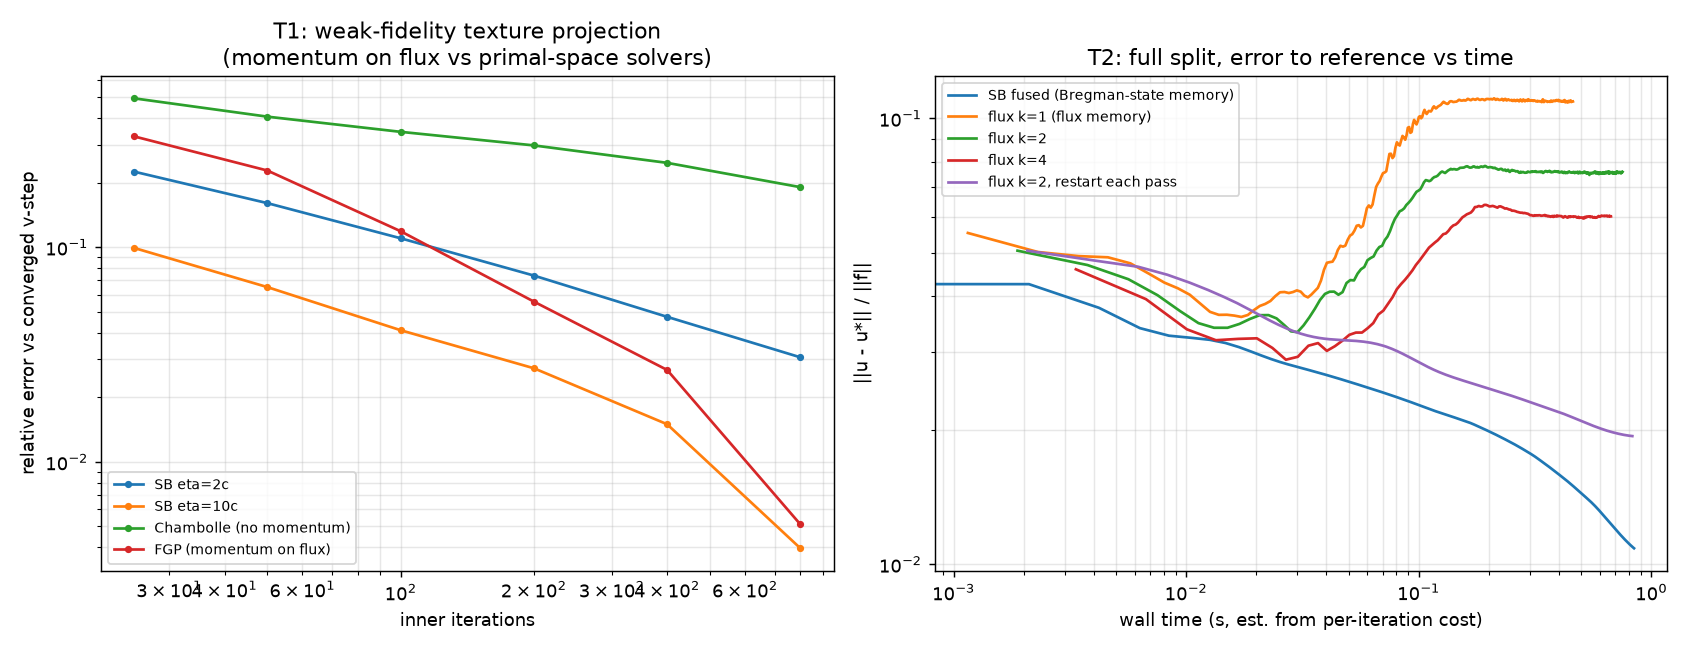
\includegraphics[width=\textwidth]{meyer_transport.png}
\caption{Left: the weak-fidelity texture projection under four solvers.
Right: full-pipeline error to the reference fixed point against wall time.}
\label{fig:transport}
\end{figure}

\section{The scale geometry of the $G$-axis}
\label{sec:softrung}

A natural extension of the decomposition is a scale ladder: rungs
$\mu_0>\mu_1>\dots>\mu_K$ and texture bands defined as differences of the
ROF scale space,
\begin{equation}
s_k=\ROF(v,1/\mu_k),\qquad
B_k = s_{k+1}-s_k,\qquad
B_K = v-s_K,
\label{eq:bands}
\end{equation}
so that $v=s_0+\sum_k B_k$. Before constructing ladders we measured the
geometry of the axis they inhabit.

\begin{measured}[The capture curve is a ramp]
\label{mr:ramp}
For a pure oscillation $g$ of $G$-norm $G$, the captured fraction
$\norm{\PG(g)}_2/\norm{g}_2$ as a function of $\mu/G$ has 10--90\%
transition width $e^{2.2}$ to $e^{2.6}$, i.e.\ $9$--$14\times$ in $\mu$,
for periods 4, 8, and 16 pixels alike (Figure~\ref{fig:transition}).
\end{measured}

This is the width that theory assigns: ROF acts on an oscillation by
soft-thresholding its amplitude, so the captured fraction is approximately
$\min(1,\mu/G)$ --- a linear ramp, whose 10--90 width is $9\times$ exactly.
Three consequences follow, each verified on the two-texture scene of
Section~\ref{sec:protocol}.

\begin{lemma}[Routing telescopes]
\label{lem:telescope}
Let bands be defined by \eqref{eq:bands} and let a two-way separation
assign each band to one of two layers by a threshold on its rung interval.
Then the layers depend only on the scale-space values at the two rungs
adjacent to the threshold; every interior rung cancels.
\end{lemma}

\begin{proof}
The sum of consecutive bands telescopes:
$\sum_{k=j}^{m-1}B_k=s_m-s_j$.
\end{proof}

Indeed, ladders of ratio 2 and ratio 4 over the same span produce
bitwise-identical two-way layers in our measurements. Consequently the
design of a two-way separation reduces to the placement of a single
straddling rung; and because the capture curve is a wide ramp rather than a
step, the optimal placement is not the geometric midpoint of the two
texture scales. On the two-texture scene, a rung at $0.79\,G_{\mathrm{fine}}$
yields total cross-leakage $0.20/0.37$ (coarse layer evaluated in the fine
texture's region and conversely), against $0.14/0.65$ for the midpoint
rung: the skewed placement is superior because the coarse texture's ramp
value at a low rung is smaller than the fine texture's ramp value at the
midpoint.

The axis is, moreover, shallow. Cross-talk between bands decays only
linearly in scale separation, so a clean separation requires a pair ratio
comparable to the transition width, approximately $14\times$; and the
usable span is bounded above by collision with the cartoon scale. When the
coarse texture's period was raised to 48 pixels ($G=153$) and $\mu$ raised
accordingly, the $u/v$ decomposition itself degraded by 6.8\,dB: the
$G$-ball at that radius absorbs cartoon structure. Between the ramp below
and the cartoon above, the $G$-axis of a $256^2$--$512^2$ image supports
approximately two genuinely separable texture bands.

We record that the opposite result was expected. In the precursor program
(Section~\ref{sec:origins}) we had established a sharp-cell ladder theorem
for windowed-spectral constraint families: geometric ladders of scale ratio
4 cover their span without interior holes, ratio 8 collapses, and a
critical ratio therefore exists in $(4,8]$. The present measurements locate
the boundary of that theorem's validity. Sharp cells are a property of the
analyzing family, not of multiscale decomposition as such; on the $G$-axis
there is no cell, no hole, and no critical ratio. Sharp multi-band texture
routing therefore belongs to windowed-spectral families, while the
$G$-ladder yields graded bands.

\begin{figure}[t]
\centering
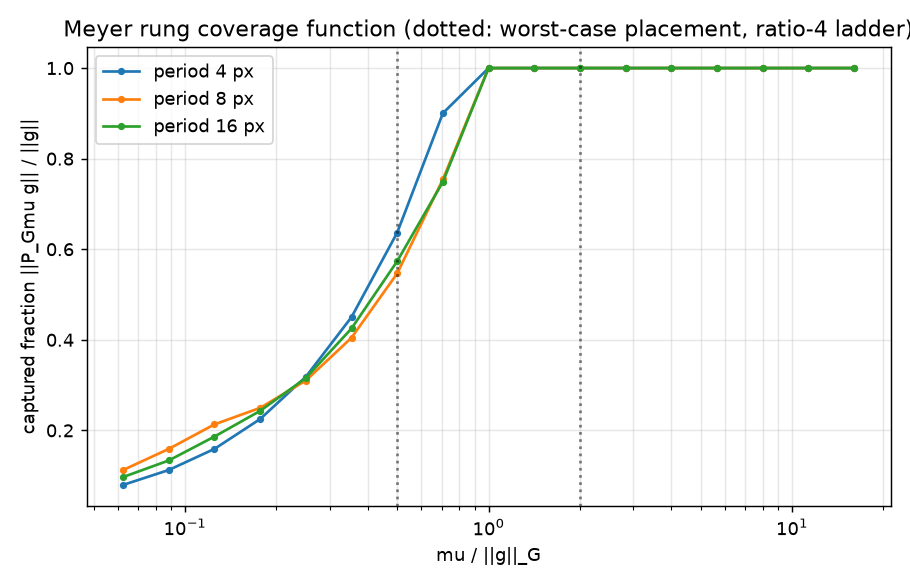
\includegraphics[width=0.72\textwidth]{meyer_transition.png}
\caption{The capture fraction of a pure oscillation under $\PG$ against
$\mu/\norm{g}_G$, for three periods. Dotted lines mark the worst-case rung
placements of a ratio-4 ladder.}
\label{fig:transition}
\end{figure}

\section{Band separation on Barbara}
\label{sec:quarantine}

Figure~2 of \cite{gilles} exhibits the standing artifact of the
single-$\mu$ model: contours of the cartoon --- the face line, the table
edge --- appear in the texture layer, because a single $G$-ball cannot
distinguish a sharp edge from a high-amplitude oscillation. A graded ladder
does not remove this leakage; it sorts it.

\begin{measured}[Barbara, rungs $\mu=\{40,10,2.5\}$]
\label{mr:bands}
On the converged texture layer, the band energies divide 5365 / 3338 /
1589, with 17 units of coarsest survivor returned to the cartoon. The
contour-leakage content concentrates in the coarse band
($\mu\,40\!\to\!10$); the mid band ($\mu\,10\!\to\!2.5$) contains the
textile content --- scarf stripes and tablecloth check --- with little
contour contamination; the fine band contains weave detail and grain
(Figure~\ref{fig:zooms}). The cost is three independent ROF solves, 1.8\,s
at $512^2$.
\end{measured}

A consumer of texture information reads the mid band and receives a layer
that the single-$\mu$ decomposition cannot produce at any parameter
setting, since its $v$ mixes the three bands by construction. The bands
must be computed as independent solves; this is the warm-state scope law of
Section~\ref{sec:polarity} in operation, since a Bregman state carried
across rungs pins the next solve at the previous fixed point and empties
the corresponding band.

\begin{figure}[t]
\centering
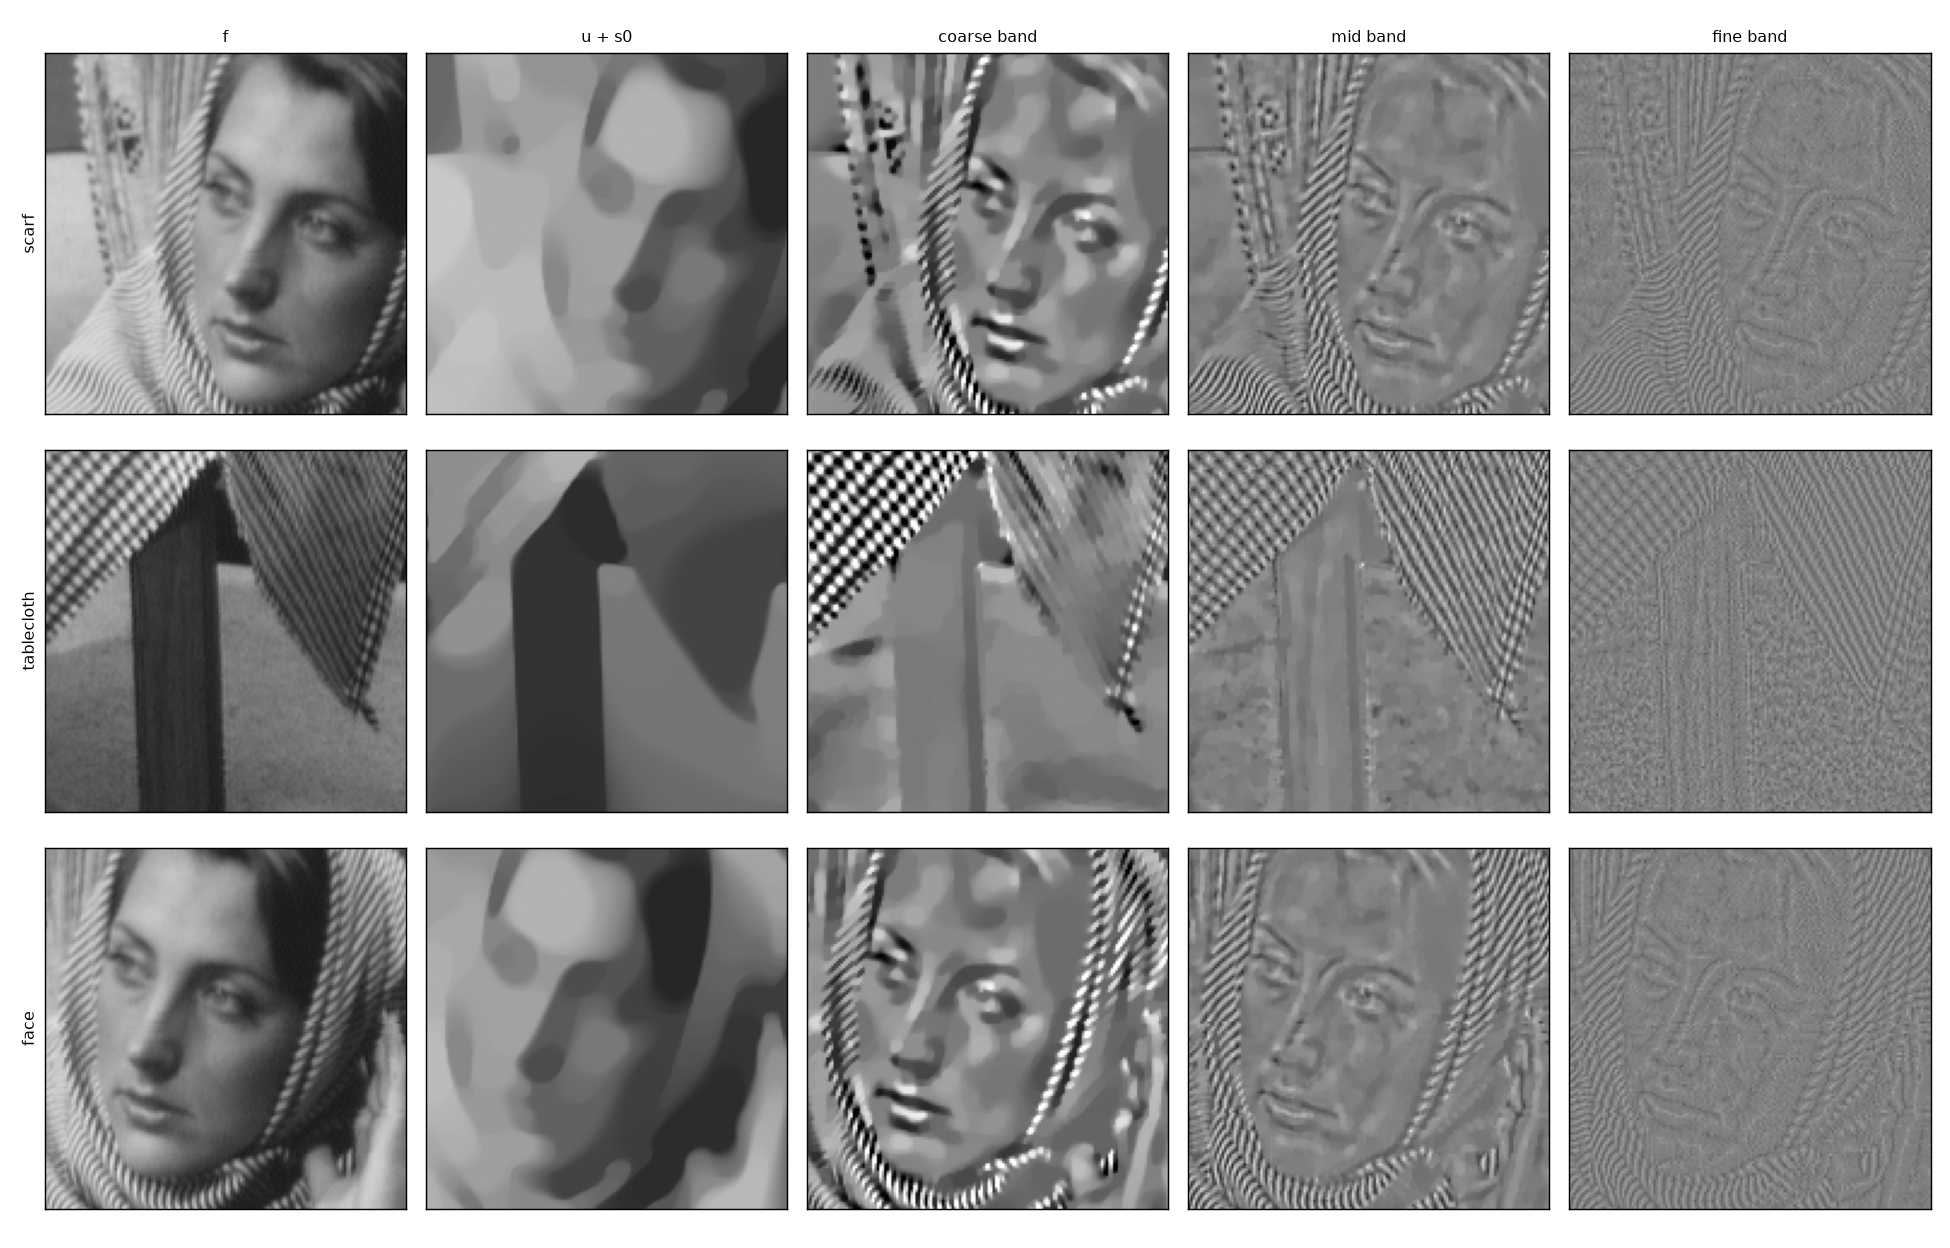
\includegraphics[width=\textwidth]{meyer_barbara_zooms.png}
\caption{Ladder bands on Barbara in three regions. Columns: input; cartoon
plus coarsest survivor; coarse band ($\mu\,40\!\to\!10$); mid band
($\mu\,10\!\to\!2.5$); fine band. Contour leakage resides in the coarse
band; the mid band carries the textile.}
\label{fig:zooms}
\end{figure}

\section{Origins of the method}
\label{sec:origins}

The method presented above is an application of principles measured in a
precursor program on time-frequency analysis. We give that history in terms
of the questions that drove it, the mathematical settings in which each
question was posed, and the truths that emerged; the reader needs no
familiarity with the program, and the statements below are quantitative.
Transport-geometric objects recur throughout it, first on the display side,
then as a rejected alternative for fusion, and finally --- in the present
paper --- as the carrier of acceleration; this recurrence, and not any
single result, is what the method's name commemorates.

\subsection{Fusion as intersection}

The program began with a question about spectrogram displays of sampled
radio signals: a long analysis window resolves frequency and blurs time, a
short window resolves time and blurs frequency; both are computed from the
same record; can one produce a display with the strengths of both?

The prevailing answers operate on the displays. Barycentric fusion computes
an optimal-transport interpolant between the two spectrograms treated as
nonnegative measures \cite{otfusion}: mass is moved between the two
pictures under structured transport costs until a compromise picture is
reached. When considering this family of methods we observed that the
compromise object is generally not the spectrogram of any signal; the
transport prior supplies the joint time-frequency structure that neither
display contains.

We instead posed the problem in the signal domain. Let $A_1,A_2$ be the
windowed Fourier analysis operators of the two window lattices, and let
$m_i=|A_i z|$ be the measured magnitudes of the record $z$. Each
measurement defines a constraint family
\[
M_i=\{\,x:\;|A_i x|=m_i\,\},
\]
and the natural fusion is an element of $M_1\cap M_2$, sought by
alternating the Griffin--Lim projection pair \cite{griffinlim}
\[
P_i(x)=A_i^{+}\bigl(m_i\cdot A_i x/|A_i x|\bigr),
\]
where $A_i^+$ is the least-squares synthesis. Three measurements fixed the
program's direction. First, the record $z$ is an exact fixed point of the
alternation: the residual at $z$ is zero to machine precision, and
therefore fusion of complementary measurements is intersection of
constraint families in the latent space rather than compromise between
displays. Second, the interference structure carries the joint information:
for two tones separated by less than the long window's resolution, the
short-window magnitudes contain the beating term that the long window
suppresses, and a controlled rotation experiment showed the short family
constrains the pair's relative phase twice as strongly as the long family.
The joint time-frequency content that barycentric methods supply by prior
is, in the signal domain, measured data. Third, the iteration's cost
structure is bimodal: from a cold start the alternation stagnates (residual
contraction $0.996$--$0.998$ per iteration), while from a physically
informed initialization it converges essentially in one step (fidelity
$0.81\to0.93$ in a single iteration, $0.99$ by 24). The initialization
purchases the basin; the projections purchase joint consistency. Heavy-ball
extrapolation at $\beta=0.88$ measurably accelerated both regimes of these
nonconvex radial projections --- the datum that Measured
Result~\ref{mr:polarity} later inverted in the convex setting.

\subsection{Coverage governs, operators polish}

The same algebra was then applied to images: two windowed-DFT patch
families --- large patches resolving spatial frequency, small patches
resolving localization --- with nonnegativity, fusing two degraded captures
of one scene. On a scene constructed so that each family resolves what the
other cannot, the fusion reached 28.5\,dB where either family alone reached
21--23\,dB. The question then became: what governs the attainable gain?

A sequence of controlled-blur studies answered it. Two captures through
identical blurs yield exactly no gain --- the method does not hallucinate.
Two captures through complementary blurs (orthogonal motion kernels) yield
a reconstruction better than either capture, recovering structure neither
contains alone. Upgraded splitting operators --- Douglas--Rachford and
relaxed variants --- yield nothing when the residual error lies in
frequency bands that no capture measured, and yield $+2.4$\,dB in a
matched problem whose error was of optimization type. Therefore recovery
quality tracks the spectral coverage of the capture set, and operator
machinery only polishes toward what is covered. The methodological
corollary --- measure the geometry of the constraint axis before building
machinery upon it --- dictated the order of operations in
Section~\ref{sec:softrung}, where the capture curve was measured first and
correctly predicted that no operator on the $G$-axis routes scales sharply.

\subsection{Ladders and their cells}

The coverage law raised a design question: how many constraint families,
at which scales, cover a working range? For windowed-spectral families the
answer sharpened into a theorem. The strength with which a window of length
$N$ constrains a component pair separated by $(\Delta t,\Delta f)$ is a
computable spectrogram overlap (log-log correlation $0.9995$ against a
closed form over three decades of scale), and geometric window ladders of
scale ratio 4 cover their span with no interior holes while ratio 8
collapses to a measured zero; a critical ratio therefore exists in $(4,8]$,
and the number of rungs required for a scale span is logarithmic.
Convergence rate obeys the same geometry: content deep within a rung's cell
converges in tens of iterations, content at a cell edge in hundreds, with
rate approximately the square of the pin strength.

These results supplied the expectations that Section~\ref{sec:softrung}
tested on Meyer's axis --- and the value of carrying a quantitative theorem
across domains is precisely that its failure is informative. The $G$-ball
capture curve is a ramp, not a cell; the critical-ratio phenomenon is a
property of windowed-spectral analysis, not of multiscale decomposition;
and the correct design rule on the $G$-axis (a single skewed straddling
rung) is different in kind from the correct rule on the spectral axis (a
logarithmic ladder at ratio 4).

\subsection{The present work}

Proposition~\ref{prop:reduction} identifies the Gilles--Osher algorithm as
a member of the class the program had characterized: an alternation of
projections onto two measured constraint families of one latent image. The
transfer of each principle then produced the results above. The
interleaving law transferred directly and yielded the $400\times$ of
Measured Result~\ref{mr:barbara}. The momentum law transferred with
reversed polarity: the $\beta=0.88$ gain of the nonconvex setting became
the divergence of Table~\ref{tab:iters}, and the question of where the
impulse belongs was settled by the problem's own transport structure ---
Meyer's norm is a flux norm, the dual variable is the flux, and
extrapolation of that flux is sound and fast (Measured
Result~\ref{mr:polarity}). The coverage-before-machinery rule dictated
measuring the capture curve before building ladders, which prevented a
class of constructions that could not have worked and produced the band
separation that does (Measured Result~\ref{mr:bands}). Each transfer was a
measurement; where the precursor law held, we used it, and where it failed,
the failure localized the law's domain of validity.

\section{Conclusion}

Algorithm 3 of \cite{gilles} is a two-projector alternation, and treating
it as such reduces its cost by two orders of magnitude: one warm Split
Bregman sweep per subproblem per pass reproduces the nested decomposition
of the $512^2$ Barbara image to $10^{-2}$ in 0.9 seconds. Acceleration in
this problem resides in its transport geometry: momentum is sound on the
dual flux and unsound on the primal images; auxiliary state transfers
along one flow and not across fidelity constants; and the scale structure
of Meyer's axis is a ramp whose geometry admits graded band separation ---
sufficient to isolate the model's contour-leakage artifact in its own band
--- but not sharp multiscale routing. The decomposition, its cost, and the
laws governing both are reproducible from the equations and parameters
given in Sections~\ref{sec:prelim}--\ref{sec:protocol}.

\begin{thebibliography}{9}
\bibitem{meyer} Y.~Meyer, \emph{Oscillating patterns in image processing
and in some nonlinear evolution equations}, AMS, 2001.
\bibitem{aujol} J.-F.~Aujol, G.~Aubert, L.~Blanc-F\'eraud, A.~Chambolle,
Image decomposition into a bounded variation component and an oscillating
component, \emph{J. Math. Imaging Vision} 22 (2005) 71--88.
\bibitem{chambolle} A.~Chambolle, An algorithm for total variation
minimization and applications, \emph{J. Math. Imaging Vision} 20 (2004)
89--97.
\bibitem{goldstein} T.~Goldstein, S.~Osher, The Split Bregman method for
L1-regularized problems, \emph{SIAM J. Imaging Sci.} 2 (2009) 323--343.
\bibitem{gilles} J.~Gilles, S.~Osher, Bregman implementation of Meyer's
$G$-norm for cartoon + textures decomposition, arXiv:2410.22777, 2024.
\bibitem{beck} A.~Beck, M.~Teboulle, Fast gradient-based algorithms for
constrained total variation image denoising and deblurring problems,
\emph{IEEE Trans. Image Process.} 18 (2009) 2419--2434.
\bibitem{griffinlim} D.~Griffin, J.~Lim, Signal estimation from modified
short-time Fourier transform, \emph{IEEE Trans. Acoust. Speech Signal
Process.} 32 (1984) 236--243.
\bibitem{otfusion} A.~Valdivia, E.~Cazelles, C.~F\'evotte, Enhancing
time-frequency resolution with optimal transport and barycentric fusion of
multiple spectrograms, arXiv:2604.15055, 2026.
\end{thebibliography}

\end{document}
